\documentclass[11pt,a4paper]{article}
\usepackage[margin=2.3cm]{geometry}
\usepackage[T1]{fontenc}
\usepackage{lmodern}
\usepackage[table]{xcolor}
\usepackage{tikz}
\usetikzlibrary{arrows.meta,positioning,shapes.geometric,fit,calc}
\usepackage{enumitem}
\usepackage{booktabs}
\usepackage{tabularx}
\usepackage{titlesec}
\usepackage{fancyhdr}
\usepackage{needspace}
\usepackage[colorlinks=true,linkcolor=ink,urlcolor=accent]{hyperref}

\definecolor{ink}{HTML}{111827}
\definecolor{accent}{HTML}{D97706}
\definecolor{soft}{HTML}{F3F4F6}
\definecolor{muted}{HTML}{6B7280}
\definecolor{ok}{HTML}{059669}

\setlength{\parindent}{0pt}
\setlength{\parskip}{6pt}
\setlist{itemsep=2pt,topsep=2pt}
\titleformat{\section}{\Large\bfseries\color{ink}}{\thesection}{0.6em}{}
\titleformat{\subsection}{\large\bfseries\color{accent}}{\thesubsection}{0.6em}{}
\pagestyle{fancy}\fancyhf{}
\renewcommand{\headrulewidth}{0.4pt}
\fancyhead[L]{\small\color{muted}SignalForge --- AI Growth Ops Engine}
\fancyhead[R]{\small\color{muted}Purpose \& Positioning}
\fancyfoot[C]{\small\color{muted}\thepage}

\newcommand{\pill}[1]{\colorbox{soft}{\strut\,#1\,}}

\begin{document}

% ------------------------------------------------------------------ title
\begin{center}
{\fontsize{26}{30}\selectfont\bfseries\color{ink} Signal\color{accent}Forge}\\[4pt]
{\large AI Growth Ops Engine for prop-trading firms, brokers and fintechs}\\[10pt]
{\color{muted}Purpose, architecture, value and go-to-market\quad|\quad Version 1.0}\\[2pt]
{\color{muted}Prepared for demonstration purposes}
\end{center}
\vspace{4pt}\hrule\vspace{8pt}

% ------------------------------------------------------------------ 1
\section{Executive summary}
SignalForge is a ready-to-run automation product that does the daily growth and operations work of
a small marketing-and-ops team for a trading brand. It is built on \textbf{n8n} (workflow
automation), \textbf{Google Gemini} (AI), \textbf{Google Sheets}, \textbf{Gmail} and
\textbf{Telegram}, plus a live web dashboard (``Mission Control'') backed by a managed MySQL database.

It runs four autonomous pipelines: it turns market news into ready-to-publish content, scores and
answers new leads within seconds, watches a target website and its public reputation around the clock,
and reports its own failures. The client configures a handful of values (brand name, site to watch,
keys) and the whole system is live. The running cost of the infrastructure is close to zero because
every component has a free tier.

\begin{center}
\begin{tabularx}{\linewidth}{>{\columncolor{soft}}X>{\columncolor{soft}}X>{\columncolor{soft}}X}
\textbf{\color{accent}Faster} & \textbf{\color{accent}Cheaper} & \textbf{\color{accent}Always on}\\
Leads answered in seconds, content briefs ready before the team starts work. &
Replaces repetitive manual work; software stack runs on free tiers. &
Scheduled and event-driven; alerts on downtime or failure without anyone watching.
\end{tabularx}
\end{center}

% ------------------------------------------------------------------ 2
\section{The problem it solves}
Trading brands (prop firms, forex and crypto brokers, fintech apps) compete in a fast, content-hungry,
trust-sensitive market. Typical pain points:
\begin{itemize}
  \item \textbf{Content treadmill.} Markets move daily; social posts, newsletters and blog ideas must follow, yet writing them is slow and repetitive.
  \item \textbf{Slow lead response.} Interested traders contact the firm at any hour. Replies that arrive hours later convert far worse than replies that arrive in minutes, and sales staff cannot tell hot leads from tyre-kickers without reading each one.
  \item \textbf{Blind spots.} A website outage during a promotion, or a sudden drop in public review score, is expensive and often noticed late.
  \item \textbf{Scattered data.} Leads, briefs and uptime checks live in inboxes and chat threads, so nobody has one view of what the automation did.
\end{itemize}

% ------------------------------------------------------------------ 3
\section{What SignalForge does: four pipelines}
\renewcommand{\arraystretch}{1.25}
\begin{tabularx}{\linewidth}{@{}p{2.6cm}p{2.5cm}X@{}}
\toprule
\textbf{Pipeline} & \textbf{Trigger} & \textbf{What happens}\\
\midrule
\textbf{A. Market intel \& content} & Daily 08:00, or manual button &
Reads three finance RSS feeds and one target web page; Gemini writes a market brief, sentiment (risk-on / risk-off / mixed), content angles, ready-to-post X, LinkedIn and Discord copy, and a blog title with SEO keywords; a second Gemini call drafts a full blog outline. Results go to Google Sheets, e-mail, Telegram and the dashboard.\\
\addlinespace
\textbf{B. Lead intake \& scoring} & Webhook (HTTP POST) &
Validates the payload, asks Gemini to score the lead 1--10, classify the trader persona, recommend a challenge size and draft a personalised reply. Hot leads (score $\geq 7$) trigger an instant Telegram alert and a priority e-mail; others get a nurture e-mail. The caller receives the scoring as JSON.\\
\addlinespace
\textbf{C. Site \& reputation monitor} & Hourly &
Checks that the target site is reachable, reads its public review score, logs uptime, and sends a Telegram alert and incident row if the site is down.\\
\addlinespace
\textbf{D. Error handler} & Any failure &
Catches failures in the other pipelines and sends Telegram and e-mail alerts naming the failed step and execution link.\\
\bottomrule
\end{tabularx}

% ------------------------------------------------------------------ 4
\section{Architecture}
\begin{center}
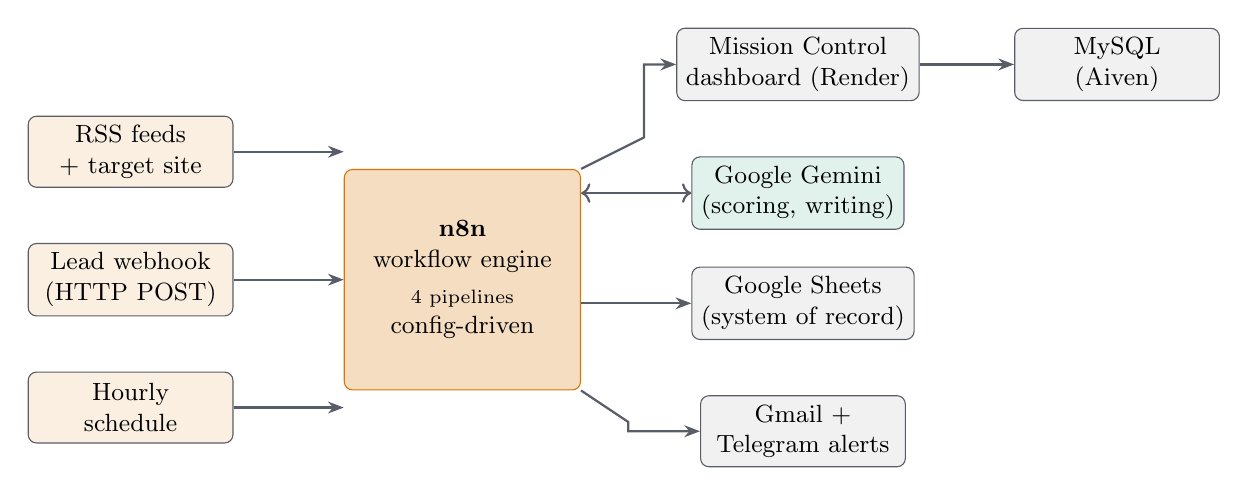
\begin{tikzpicture}[
  node distance=7mm and 9mm,
  box/.style={rounded corners=3pt,draw=ink!70,fill=soft,align=center,minimum height=9mm,minimum width=26mm,font=\small},
  src/.style={box,fill=accent!12},
  ai/.style={box,fill=ok!12},
  outb/.style={box,fill=ink!6},
  arr/.style={-{Stealth[length=2mm]},draw=ink!70,thick}]
  \node[src] (rss) {RSS feeds\\+ target site};
  \node[src,below=of rss] (hook) {Lead webhook\\(HTTP POST)};
  \node[src,below=of hook] (cron) {Hourly\\schedule};
  \node[box,right=14mm of hook,minimum height=28mm,minimum width=30mm,fill=accent!25,draw=accent] (n8n) {\textbf{n8n}\\workflow engine\\[2pt]\scriptsize 4 pipelines\\config-driven};
  \node[ai,right=14mm of n8n,yshift=11mm] (gem) {Google Gemini\\(scoring, writing)};
  \node[outb,right=14mm of n8n,yshift=-3mm] (sheet) {Google Sheets\\(system of record)};
  \node[outb,below=of sheet] (mail) {Gmail +\\Telegram alerts};
  \node[outb,above=of gem] (dash) {Mission Control\\dashboard (Render)};
  \node[outb,right=10mm of dash,xshift=2mm] (db) {MySQL\\(Aiven)};
  \draw[arr] (rss) -- (n8n.west|-rss.east);
  \draw[arr] (hook) -- (n8n);
  \draw[arr] (cron) -- (n8n.west|-cron.east);
  \draw[arr,<->] (n8n.east|-gem) -- (gem);
  \draw[arr] (n8n.east|-sheet) -- (sheet);
  \draw[arr] (n8n.south east) -- ++(6mm,-4mm) |- (mail);
  \draw[arr] (n8n.north east) -- ++(8mm,4mm) |- (dash);
  \draw[arr] (dash) -- (db);
\end{tikzpicture}
\end{center}
\textit{Data flow:} triggers feed n8n; n8n calls Gemini for intelligence; results are written to Google
Sheets (human-readable record), pushed to the dashboard database (live view) and sent to people by
e-mail and Telegram.

% ------------------------------------------------------------------ 5
\section{Technology choices and why}
\begin{tabularx}{\linewidth}{@{}p{3.1cm}X@{}}
\toprule
\textbf{Component} & \textbf{Role and reason for choosing it}\\
\midrule
\textbf{n8n} & Visual workflow engine. Each step is inspectable, retries and error routing are built in, and non-developers can adjust a flow. Hosted in n8n Cloud here; self-hostable for free for clients who need data residency.\\
\addlinespace
\textbf{Google Gemini API} & The AI layer for scoring, summarising and writing. Chosen for its generous free tier, JSON-mode output (reliable structured results) and strong quality on short-form business writing.\\
\addlinespace
\textbf{Google Sheets} & Zero-setup system of record that the client's team already knows how to filter, share and chart. Every action is logged as a row.\\
\addlinespace
\textbf{Gmail} & Delivers briefs, lead replies and error reports from a normal business mailbox with OAuth sign-in (no passwords stored in the workflow).\\
\addlinespace
\textbf{Telegram bot} & Instant push alerts to a phone at no cost; ideal for ``hot lead'' and ``site down'' moments where speed matters.\\
\addlinespace
\textbf{Mission Control dashboard} & Hono/React web app on Render that gives a live, shareable view of briefs, leads and uptime. It is the part clients show to colleagues.\\
\addlinespace
\textbf{Aiven MySQL} & Managed database behind the dashboard: encrypted connections, backups and a free development tier.\\
\addlinespace
\textbf{GitHub} & Version control for the workflow export, dashboard code and documentation, so every client deployment is reproducible.\\
\bottomrule
\end{tabularx}

% ------------------------------------------------------------------ 6
\section{Benefits to the user}
\begin{itemize}
  \item \textbf{Speed to lead.} Every lead is scored, answered and routed in seconds, around the clock, so the best prospects are never left waiting.
  \item \textbf{Consistent content.} A daily brief and publish-ready copy arrive every morning, tied to what actually moved markets.
  \item \textbf{Early warning.} Downtime and reputation changes surface as phone alerts within the hour.
  \item \textbf{One source of truth.} Sheets for analysts, dashboard for managers, Telegram and e-mail for action.
  \item \textbf{Low cost and low lock-in.} Free-tier infrastructure; the workflow is a portable JSON file; services can be swapped (for example another AI model or CRM).
  \item \textbf{White-label by configuration.} Brand name, monitored site, review domain, recipients and keys are settings, so onboarding a new client is a configuration task, not a rebuild.
  \item \textbf{Transparent AI use.} Each AI output is stored beside its input, so staff can review replies before scaling automatic sending.
\end{itemize}

% ------------------------------------------------------------------ 7
\Needspace{12\baselineskip}
\section{Who it is for and how to position it}
\subsection{Target customers}
Proprietary trading (funded-trader) firms, retail forex and CFD brokers, crypto exchanges and
educators, and fintech apps with a high-volume inbound lead flow and a content-driven brand.

\subsection{Positioning statement}
\begin{quote}
\textit{SignalForge is the always-on AI growth team for trading brands: it writes the daily market
content, answers and ranks every lead in seconds, and watches your site and reputation, for the cost
of a software subscription instead of a salary.}
\end{quote}

\subsection{Commercial model (illustrative)}
\begin{center}
\begin{tabularx}{\linewidth}{@{}lXl@{}}
\toprule
\textbf{Tier} & \textbf{Scope} & \textbf{Model}\\
\midrule
Starter & Pipelines A--D, one brand, shared dashboard & Setup fee + monthly\\
Growth & Adds competitor watch, CRM sync, approval-before-publish & Setup + higher monthly\\
Scale & Multi-brand, custom pipelines, SLA and reporting & Custom retainer\\
\bottomrule
\end{tabularx}
\end{center}
Prices are deliberately left to be set per market; the margin comes from reusing one configured
engine across many clients.

\subsection{Demonstration flow (about 10 minutes)}
\begin{enumerate}[label=\textbf{\arabic*.}]
  \item Open the dashboard beside the n8n canvas.
  \item Click \textit{Run Demo Now}: show feeds, AI calls and the five parallel outputs lighting up.
  \item Show the new dashboard entry, Google Sheet rows, e-mail and Telegram message.
  \item POST a sample lead; show the score, persona and drafted reply, and the hot-lead alert.
  \item Close with the configuration step: ``Change three values and this runs on your brand.''
\end{enumerate}

% ------------------------------------------------------------------ 8
\section{Roadmap}
\textbf{Next:} competitor watch across several sites; CRM sync (HubSpot or Salesforce); human approval before auto-posting.

\textbf{Then:} weekly executive report; multi-brand dashboard; compliance checks for financial promotions; multi-language content.

% ------------------------------------------------------------------ 9
\section{Operating notes and limits}
\begin{itemize}
  \item \textbf{AI output needs review at first.} Drafted replies and posts should be sampled by a person before fully automatic sending, especially for regulated financial promotion.
  \item \textbf{Secrets.} API keys live in the workflow's configuration nodes for demo speed. For production, move them to n8n credentials and rotate any keys that were shared in chat.
  \item \textbf{Free-tier limits.} Free hosting can sleep when idle, and Gemini's free tier has daily request caps; both are fine for demos and small clients, and are upgraded as volume grows.
  \item \textbf{Public data only.} Scraping is limited to public pages and public review scores; always respect each site's terms.
\end{itemize}

\end{document}
